\documentclass[12pt]{article}
\usepackage[utf8]{inputenc}
\usepackage[spanish]{babel}
\usepackage{ragged2e}
\usepackage{amsmath}
\usepackage{graphicx}
\usepackage{hyperref}
\usepackage{fancyhdr}
\usepackage{subcaption}

\title{\huge Práctica Supervisada\vspace*{5cm}}

\author{Amallo, Sofía - Gil, Juan Manuel}

\date{\parbox{\linewidth}{\centering%
  Noviembre 18, 2022 \endgraf\bigskip
  \vspace*{4cm}
  Dr. Ing. Horacio A. Mendoza \hspace*{1cm} Dr. Ing. Jorge Finochietto\endgraf\medskip
  \vspace*{0.5cm}
  Laboratorio de\ Comunicaciones Digitales \endgraf
  Universidad Nacional de Córdoba}}
  
\begin{document}

\maketitle
\thispagestyle{empty}
\newpage

%\pagestyle{myheadings}
\markright{}

\section{Ficha de Práctica Supervisada}
\subsection{Datos de los Alumnos}
\raggedright
\textsl{Nombre y Apellido:}  Sofía Amallo

\textsl{N° de Matrícula:} 41.279.731

\textsl{Teléfono:} 3512355718

\textsl{Correo electrónico:} sofia.amallo@mi.unc.edu.ar
\vspace*{0.5cm}

\textsl{Nombre y Apellido:} Juan Manuel Gil

\textsl{N° de Matrícula:} 41.592.940

\textsl{Teléfono:} 3571604632

\textsl{Correo electrónico:} juan.manuel.gil@mi.unc.edu.ar

\subsection{Datos de la Institución Receptora}
\textsl{Nombre:} Laboratorio de Comunicaciones Digitales

\textsl{Dirección del Laboratorio:} Av. Vélez Sársfield 1600 CU, Cba - Argentina

\textsl{Nombre y Apellido del Supervisor Docente:} Dr. Ing. Jorge Manuel Finochietto

\textsl{Cargo que ocupa el Supervisor Docente en la Institución Receptora:} Secretario de Tecnología  Educación Virtual, Jefe de cátedra de Informática e Investigador Independiente del CONICET

\textsl{N° de Teléfono:} (+54) 351 5353800 int 29085

\textsl{Correo Electrónico:} lcd@fcefyn.unc.edu.ar

\subsection{Datos del Tutor}

\textsl{Nombre y Apellido:} Dr. Ing. Horacio A. Mendoza

\textsl{Cargo y Cátedra:} Docente e Investigador

\textsl{Teléfono:} (+54) 351 5353800 int 29085

\textsl{Correo Electrónico:} lcd@fcefyn.unc.edu.ar

\subsection{Datos de la Práctica Profesional Supervisada}

\textsl{Fecha de Inicio:} 26/09/2022

\textsl{Fecha de Finalización:} 18/11/2022

\textsl{Total de horas:} 222

\tableofcontents
\newpage

\justifying
\section{Resumen}
\setlength\parindent{24pt}
\newpage
\section{Introducción}
La Práctica Supervisada (PS) se llevó a cabo en el Laboratorio de Comunicaciones Digitales (LCD) de la Universidad Nacional de Córdoba, Córdoba, Argentina, donde se abordó el desafío de desarrollar \textit{payloads}, tam-bién conocidas como cargas útiles, con el fin de expandir las funcionalidades del drone Matrice 300 RTK de DJI.

En ese contexto se investigaron distintas maneras de interactuar con dicho drone, siendo algunas el SDK (Software Development Kit) que brinda el fabricante que cumple el rol de una API (Application Programming Interface). Se investigó acerca del protocolo UART como solución al problema de la comunicación entre el drone y las distintas payloads.

Una de las partes mas enriquecedoras de nuestra experiencia en el labora-torio fue la dinámica de trabajo, ya que abordamos diferentes soluciones a medida que se presentaron nuevas problemáticas, algo propio del desarrollo con nuevas tecnologías como es nuestro caso. 

La curva de aprendizaje en dichas tecnologías se documentó en Notion, una plataforma de sofware orientada a la toma de notas, lo cual nos permitirá confeccionar de una manera concisa una llamada ``hoja de ruta"  que quede a disposición de otros estudiantes que transiten por el LCD, con el objetivo de brindarle alguna retribución a la institución que nos brindó herramientas de trabajo, acceso a equipos, placas e insumos para el desarrollo de nuestro trabajo y sobre todo un espacio de aprendizaje junto a docentes y compañeros. Sin dudas nuestro paso por el Laboratorio de Comunicaciones Digitales se constituyó en una de las experiencias fundamentales de nuestra formación en el campo profesional.

\vspace{1.5cm}
\begin{tabular}{p{5.5cm}cp{5.5cm}}
  \cline{1-1} \cline{3-3} \\
  \centering Estudiante   \\ Sofía, Amallo && \centering Estudiante \\ Gil, Juan Manuel
\end{tabular}

\vspace{1.5cm}

\begin{tabular}{p{5.5cm}cp{5.5cm}}
  \cline{1-1} \cline{3-3} \\
  \centering Supervisor   \\ Dr. Ing. Finochietto, Jorge M. && \centering Tutor \\ Dr. Ing. Mendoza, Horacio A.
\end{tabular}


\newpage
\section{Herramientas de trabajo}
\justifying
Para realizar las experiencias, que se describirán posteriormente en este documento, fueron necesarias algunas placas de desarrollo, las mismas se listarán en esta sección.
\subsection{PyCom}
Por un lado se utilizó hardware del fabricante \textit{PyCom}, en particular, los módulos \textit{FiPy}[Fig. 4.1 y Fig. 4.2] y su placa de expansión \textit{FyPy}[Fig. 4.3 y Fig 4.4]. La utilización de estas placas fue debido a que se proyecta que las futuras payloads que lleve el drone sean estas o similares.

\begin{figure}[ht]
  \centering
  \begin{subfigure}[b]{0.45\linewidth}
    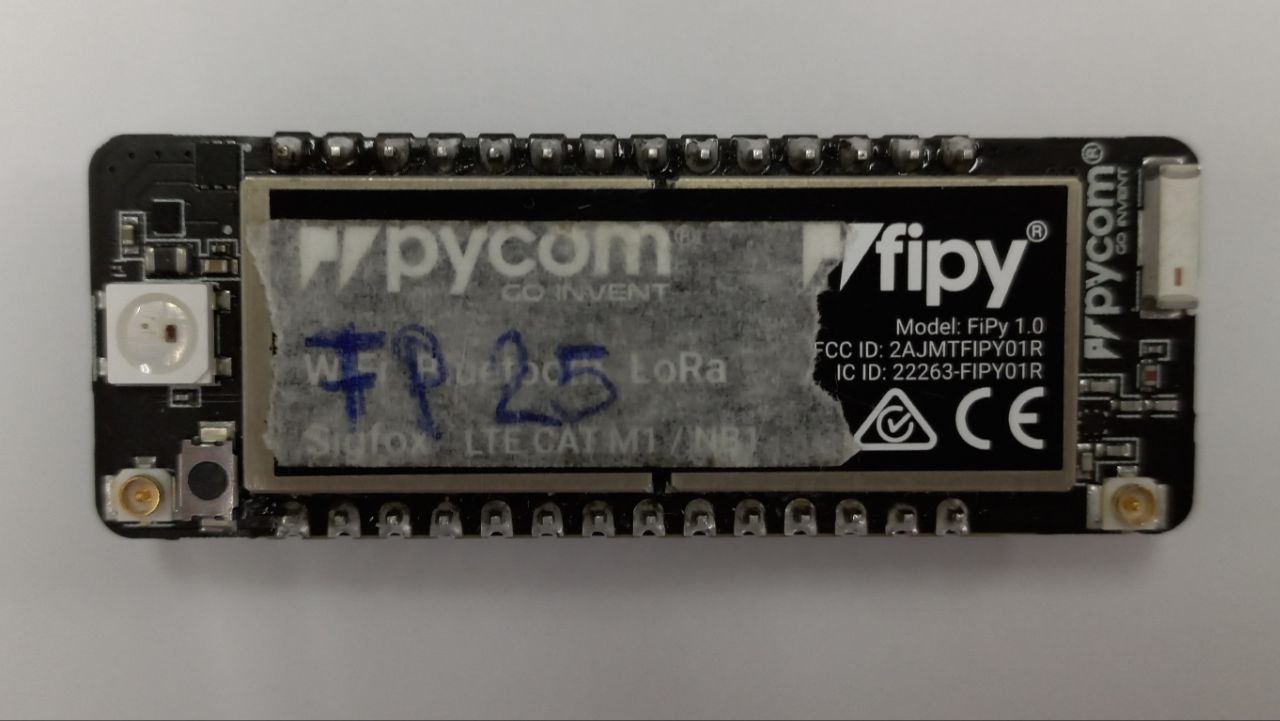
\includegraphics[width=\linewidth]{images/FiPy-1.jpg}
    \caption{Fig. 4.1: FiPy frente}
    \label{fig:FiPy-fte}
  \end{subfigure}
  \begin{subfigure}[b]{0.45\linewidth}
    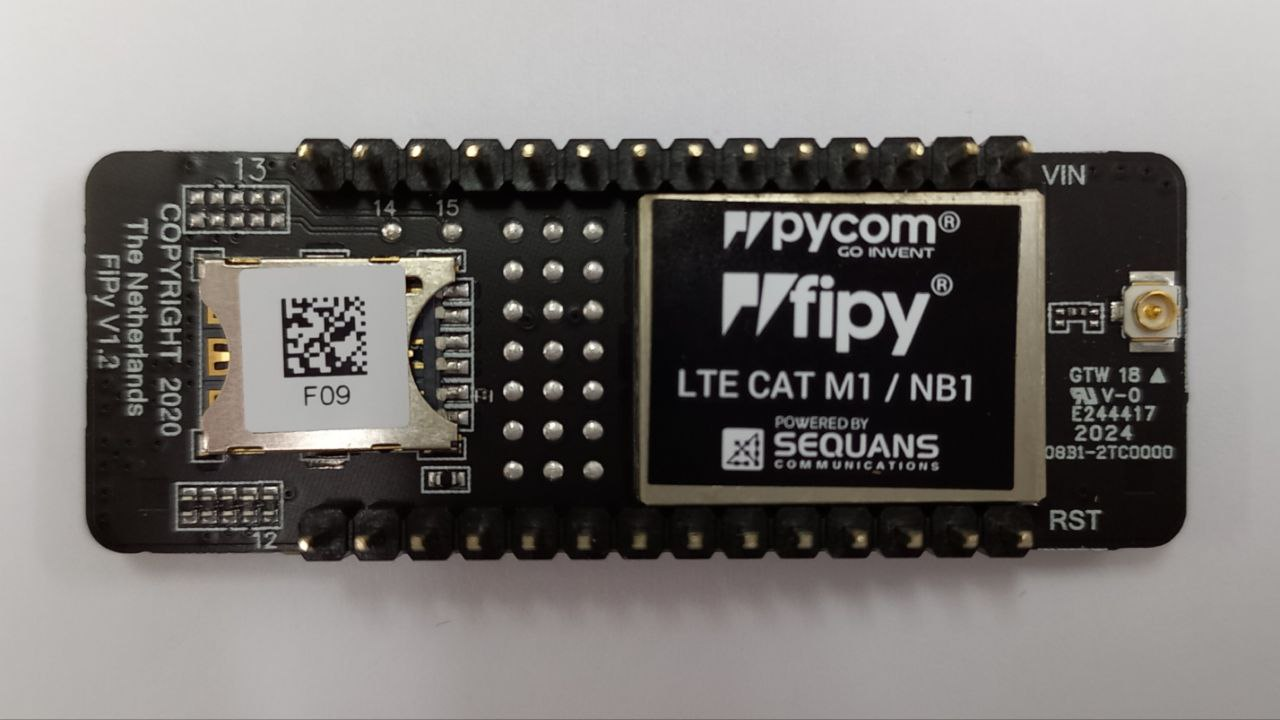
\includegraphics[width=\linewidth]{images/FiPy-2.jpg}
    \caption{Fig. 4.2: FiPy dorso}
    \label{fig:FyPy-dor}
  \end{subfigure}
  \centering
  \begin{subfigure}[b]{0.45\linewidth}
    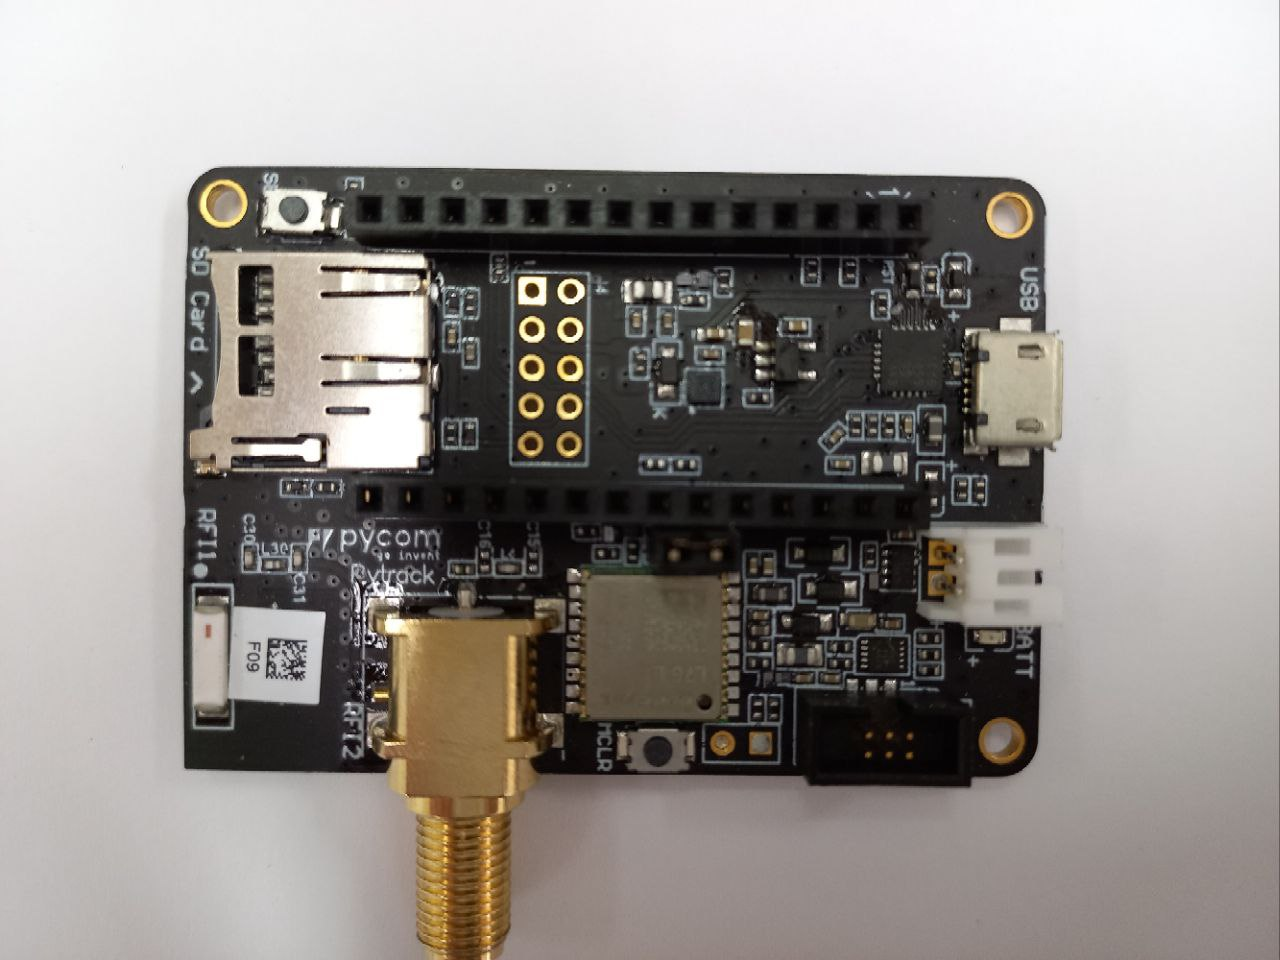
\includegraphics[width=\linewidth]{images/PyTrack-1.jpg}
    \caption{Fig. 4.3: PyTrack frente}
    \label{fig:PyTrack-fte}
  \end{subfigure}
  \begin{subfigure}[b]{0.45\linewidth}
    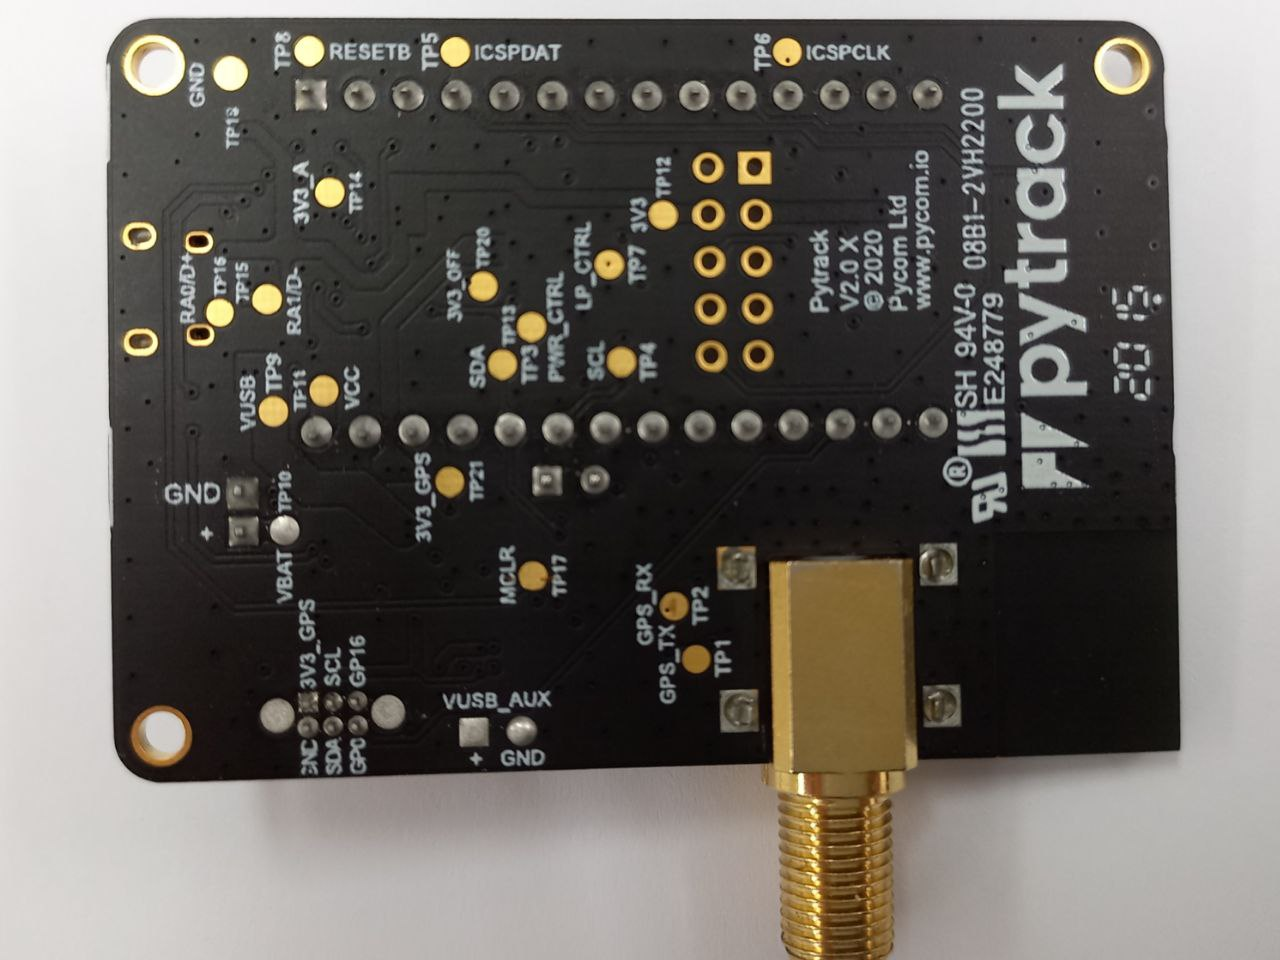
\includegraphics[width=\linewidth]{images/PyTrack-2.jpg}
    \caption{Fig. 4.4: PyTrack dorso}
    \label{fig:PyTrack-dor}
  \end{subfigure}
\end{figure}

Las \textit{PyCom} pueden trabajar con distintos módulos fábricados por terceros a través de sus pines GPIO, o utilizando sus puertos UART. También son capaces de brindar interfaces de red tales como WiFi, Bluetooth, Celular, Lora y Sigfox.

En cuanto a procesamiento cuenta con una \textit{ESP32 SoC} lo que implica un microprocesador Xtensa, con arquitectura ARM de 32-bits; dual-core, con una frecuencia de trabajo de 240MHz.

Una lista completa con todas las funcionalidades ofrecidas por los módulos puede ser consultada en el \href{https://docs.pycom.io/gitbook/assets/specsheets/Pycom_002_Specsheets_FiPy_v2.pdf}{manual de usuario de FiPy} y/o el \href{https://pycom.io/product/pytrack-2-0-x/}{manual de usuario de PyTrack}.

Ambas placas utilizan el lenguaje \href{https://github.com/micropython/micropython}{micropython} para el desarrollo, el cual es un set de funciones reducidas de los módulos originales de Python.

\subsection{SMT32F4}
Esta placa se utilizó con el objetivo de realizar pruebas tratándola como una interfaz drone-payloads, el plan era consumir del SDK del drone (escrito en c) y pasarle información a la \textit{PyCom}, al igual que, en base a los datos recopilados por la payload, darle instrucciones al UAV.
La \textit{SMT32F4} [Fig. 4.5, 4.6] es una placa que posee un procesador Cortex M4, con arquitectura ARM de 32-bit y una frecuencia de operación de 180 MHz. Nos brinda múltiples GPIO para la interacción con hardware y sensores de terceros. Si requiere indagar un poco más sobre la placa puede consultar su \href{https://drive.google.com/file/d/182H9i1qmJ2UCbynztxymEA3nfmx_eGrk/view?usp=share_link}{\textit{manual}}.

\begin{figure}[ht]
  \centering
  \begin{subfigure}[b]{0.45\linewidth}
    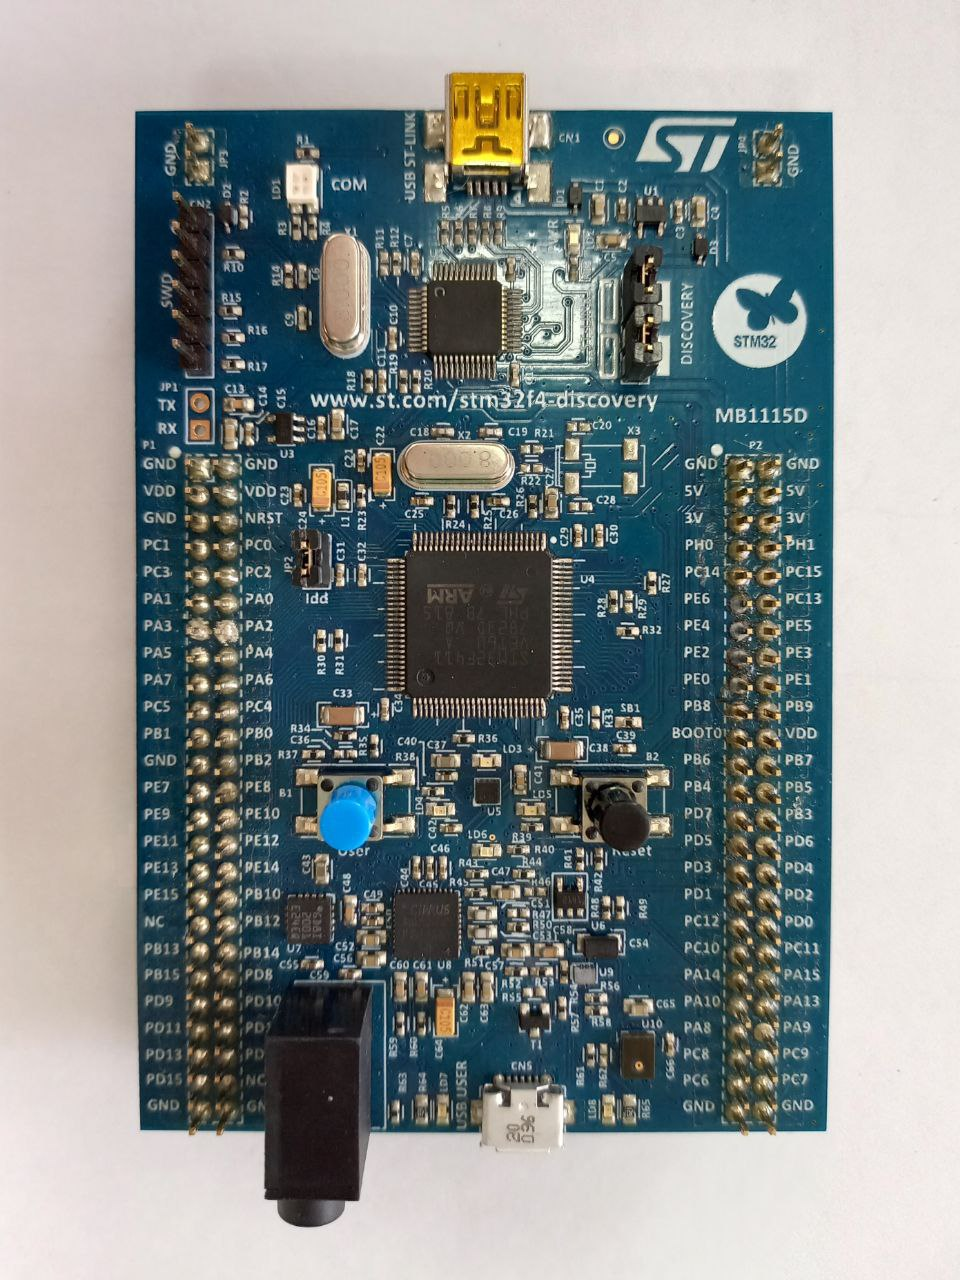
\includegraphics[width=\linewidth]{images/STM32F4-1.jpg}
    \caption{Fig. 4.5: STM32F4 frente}
  \end{subfigure}
  \begin{subfigure}[b]{0.45\linewidth}
    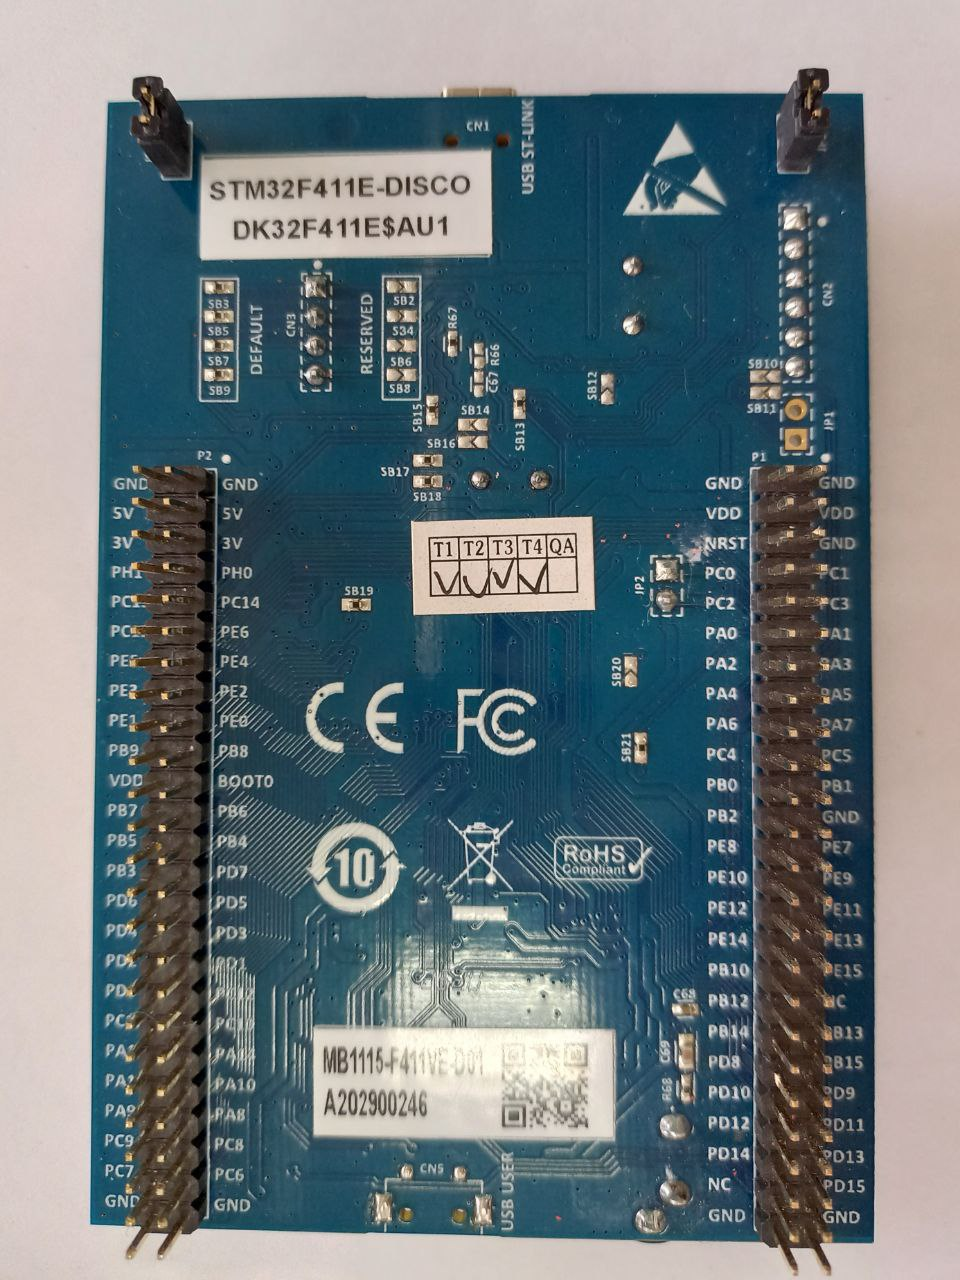
\includegraphics[width=\linewidth]{images/STM32F4-2.jpg}
    \caption{Fig. 4.6: STM32F4 dorso}
  \end{subfigure}
\end{figure}


\subsection{USB to UART}
Este adaptador se utilizó en instancias de pruebas para poder enviar datos desde la PC a las placas, o recibir desde las placas a la PC.

\begin{figure}[ht]
  \centering
  \begin{subfigure}[b]{0.45\linewidth}
    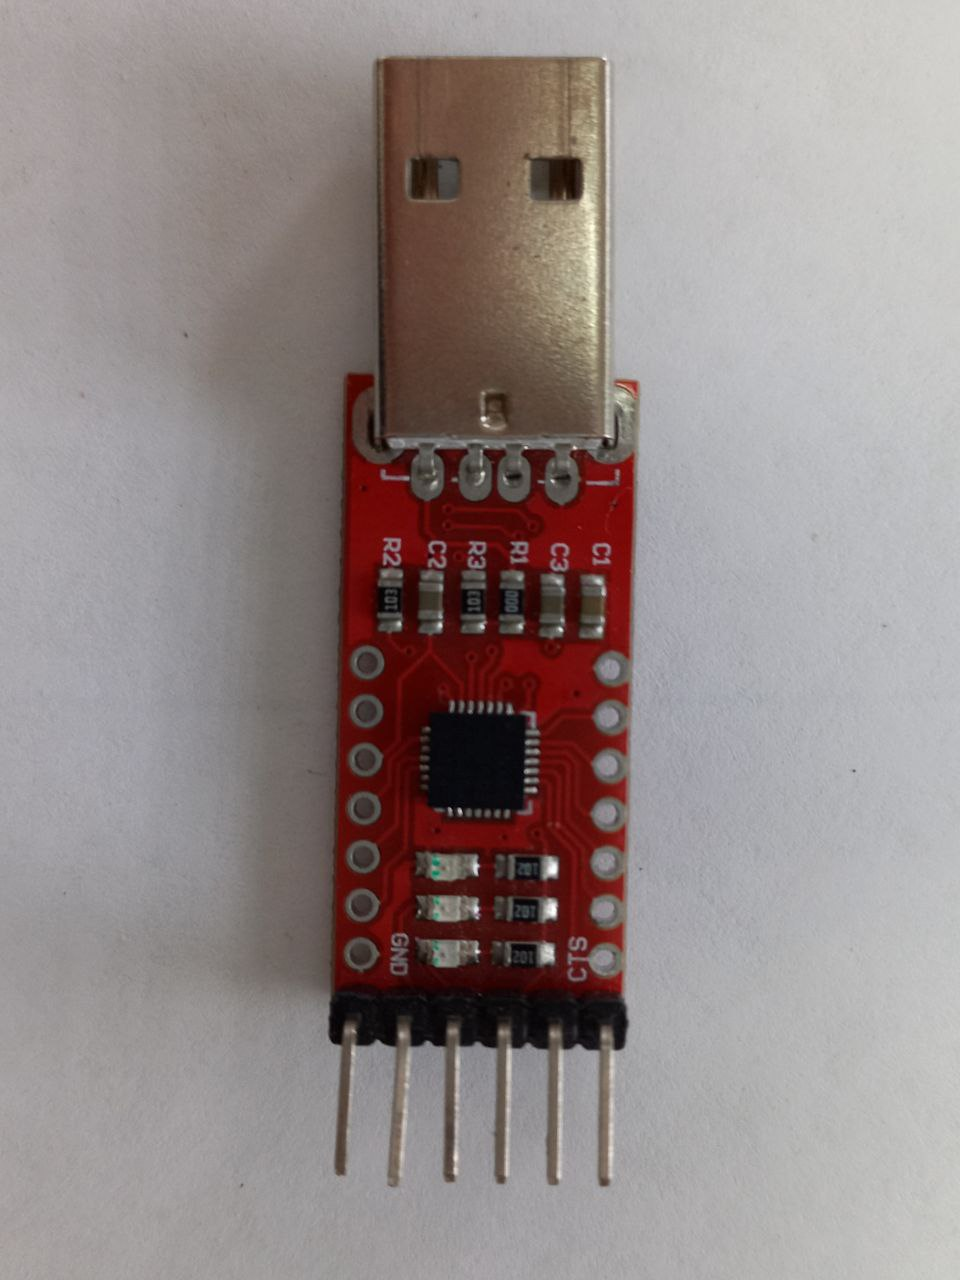
\includegraphics[width=\linewidth]{images/USB-UART-1.jpg}
    \caption{Fig. 4.7: USB to UART frente}
  \end{subfigure}
  \begin{subfigure}[b]{0.45\linewidth}
    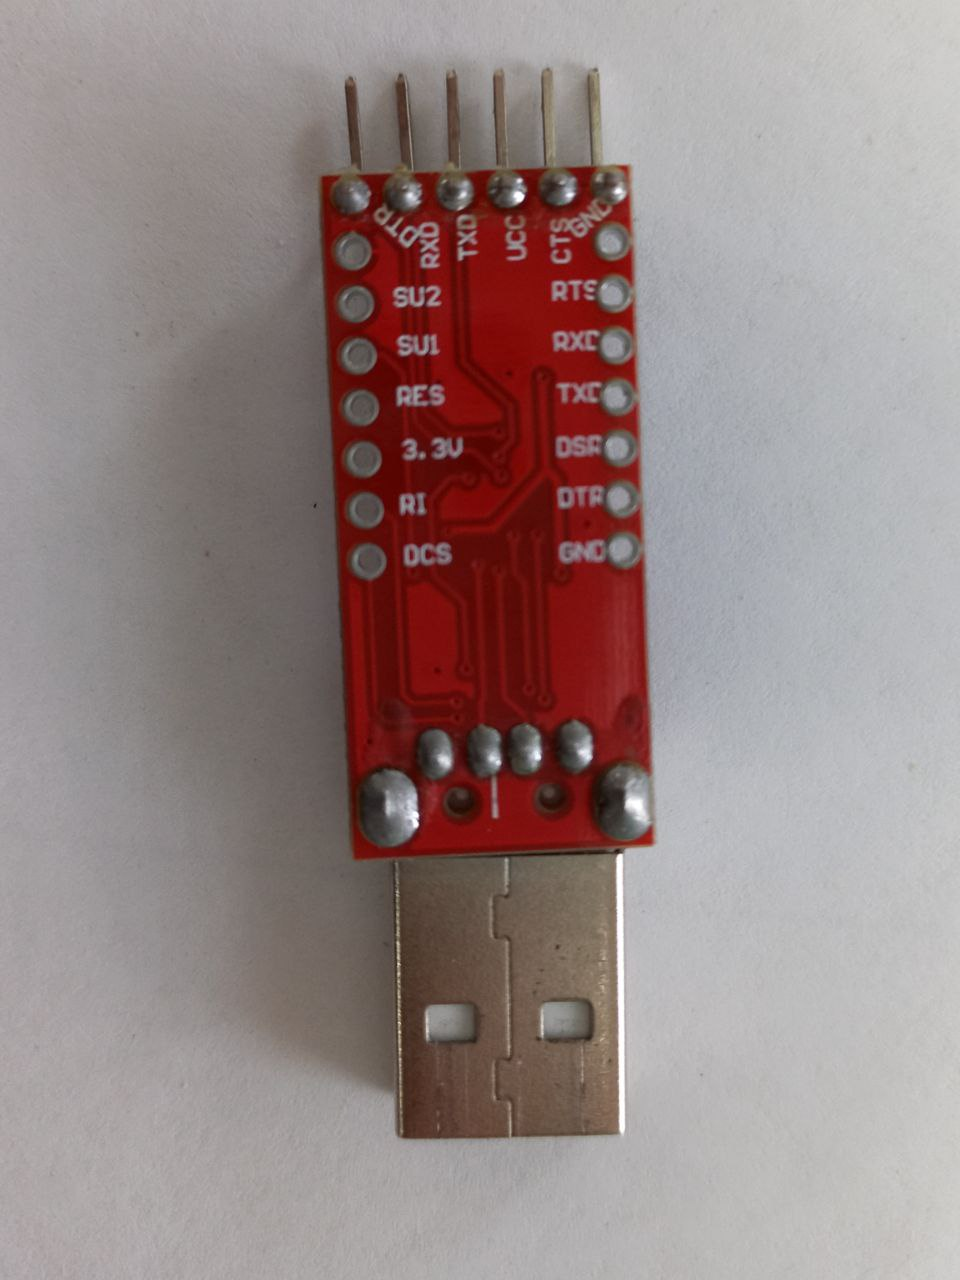
\includegraphics[width=\linewidth]{images/USB-UART-2.jpg}
    \caption{Fig. 4.8: USB to UART dorso}
  \end{subfigure}
\end{figure}

\subsection{Payload SDK Devekopment Board Kit}
La utilización de la \textit{SMT32F4} se debió a que en un primer momento no se tuvo en cuenta que el drone ya contaba con un accesorio para realizar esta tarea, la \href{https://store.dji.com/product/psdk-development-kit}{\textit{Payload SDK Devekopment Board Kit}} [Fig. 4.5, Fig. 4.6 y 4.7]
Luego de investigaciones vimos que esto es justo lo que se precisaba, ya que nos brinda una interfaz para la conexión con el drone, y una placa de desarrollo la cual también es una \textit{SMT32} con un pocesador ARM de 32-bit, no se cuenta con más detalles de dicho chip, aún así debería cubrir todas las interacciones con el SDK de DJI.

\begin{figure}[ht]
  \centering
  \begin{subfigure}[b]{0.45\linewidth}
    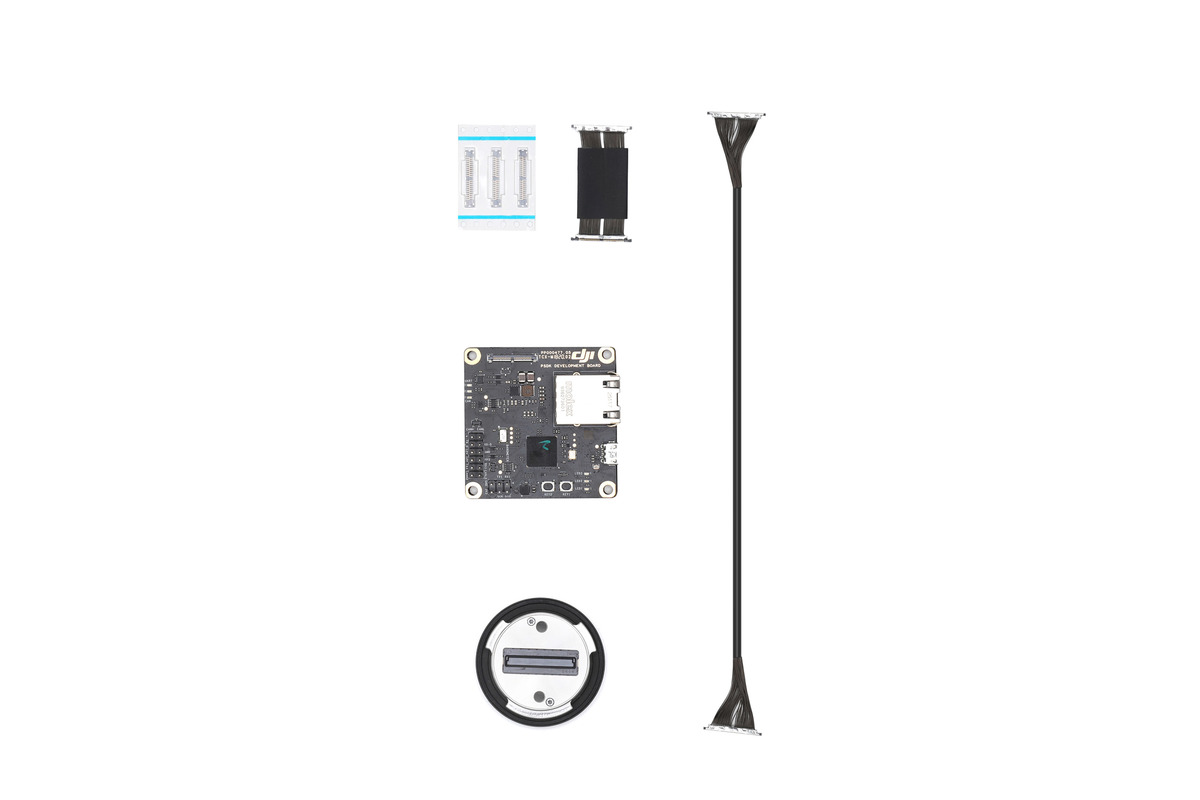
\includegraphics[width=\linewidth]{images/Payload-DBK-1.jpg}
    \caption{Fig. 4.9: kit completo}
  \end{subfigure}
  \begin{subfigure}[b]{0.45\linewidth}
    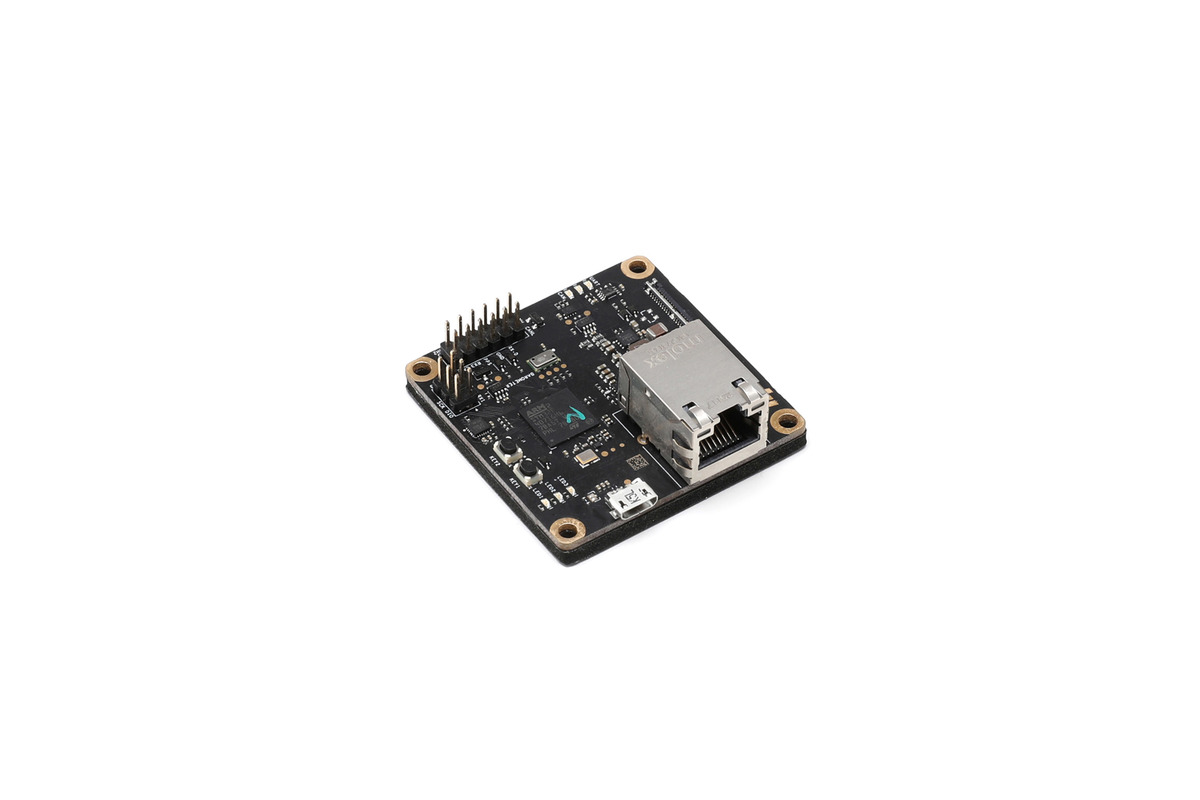
\includegraphics[width=\linewidth]{images/Payload-DBK-2.jpg}
    \caption{Fig. 4.10: Placa de desarrollo}
  \end{subfigure}
  \begin{subfigure}[b]{0.45\linewidth}
    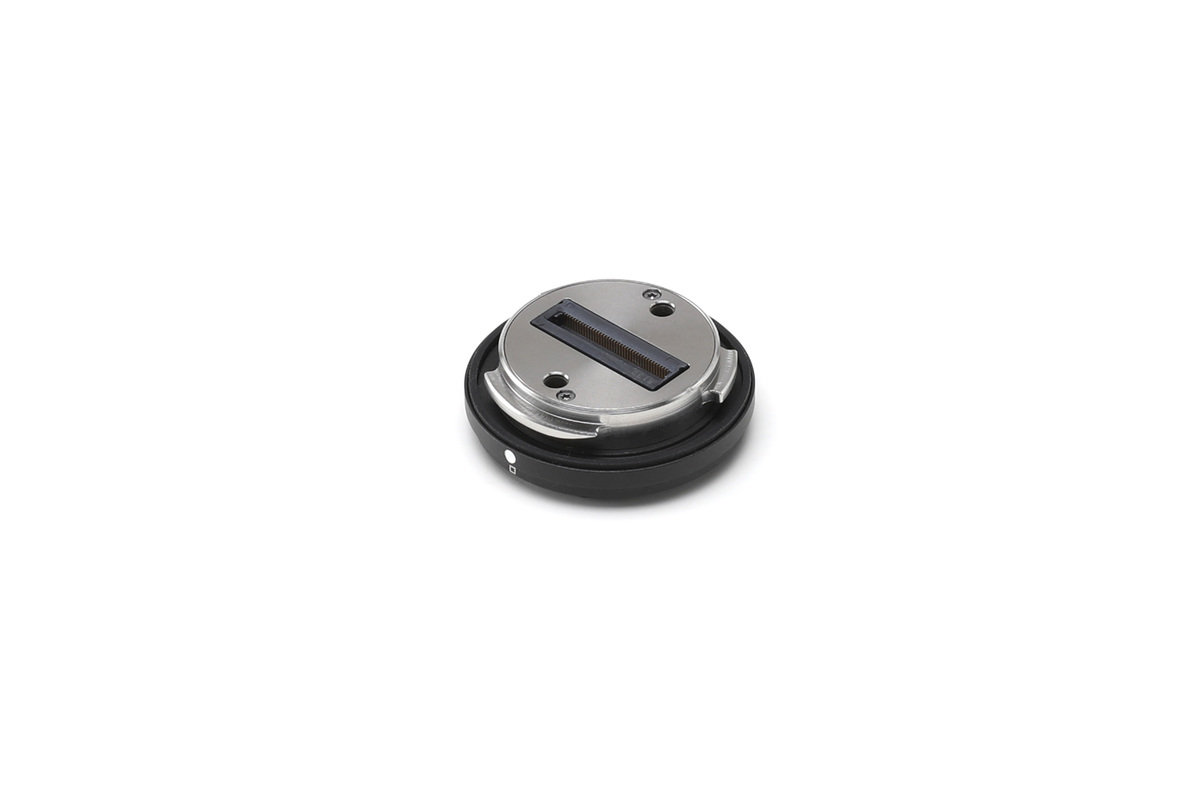
\includegraphics[width=\linewidth]{images/Payload-DBK-3.jpg}
    \caption{Fig 4.11: Conector de la interfaz}
  \end{subfigure}
\end{figure}

\vspace*{200pt}
\newpage
\section{Desafíos abordados}

\subsection{DJI SDK}
La investigación sobre el \textit{SDK} del drone nace como respuesta a la oportu-nidad de montar payloads sobre \textit{UAV}. Tener cargas útiles sobre el drone es de una gran útilidad dado que utilizando \textit{D-RTK2} se pueden obtener datos acompañados de una alta precisión que la obtenemos a través del GPS del mismo en tiempo real.

Algunas de las aplicaciones que podrían resultar de estas implementacio-nes son:
\begin{itemize}
  \item \textbf{Recolección de datos de multinodos}, en sistemas con multinodos que recopilan información, el drone puede ser una excelente opción para planificar rutas he ir recolectando e indicando a donde redireccionar los datos al mismo tiempo.
  \item \textbf{Inspección de redes de alta tensión}, permite encontrar defectos en las powerlines desde una distancia segura.
  \item \textbf{Agricultura de precisión}, ya sea para la detección de plagas, male-zas, monitorear rendimientos, intervenir en sectores específicos del cul-tivo de manera inmediata, etc.
  \item \textbf{Minería}, para inspeccionar cañerías de gas o combustible con lasers de detección de fugas.
  \item \textbf{Combate contra incendios}, se podría equipar con cámaras especiales con zoom óptico para identificar focos de fuego, planear estrategias y reconocer situaciones peligrosas.
  \item \textbf{Seguridad}, se podría utilizar para patrullaje y monitoreo de zonas conflictivas o díficiles de cubrir, como por ejemplo las fronteras.
\end{itemize}

Ahora se adjuntarán los distintos módulos que existen el el SDK de payloads provisto por DJI, estos son los que abrirán las puertas a nuevas aplicaciones, los mismos se clasifican en dos grandes subsecciones, \textit{Basic Function} o \textit{Advanced Function}.

\begin{figure}[ht]
  \centering
  \begin{subfigure}[b]{0.45\linewidth}
    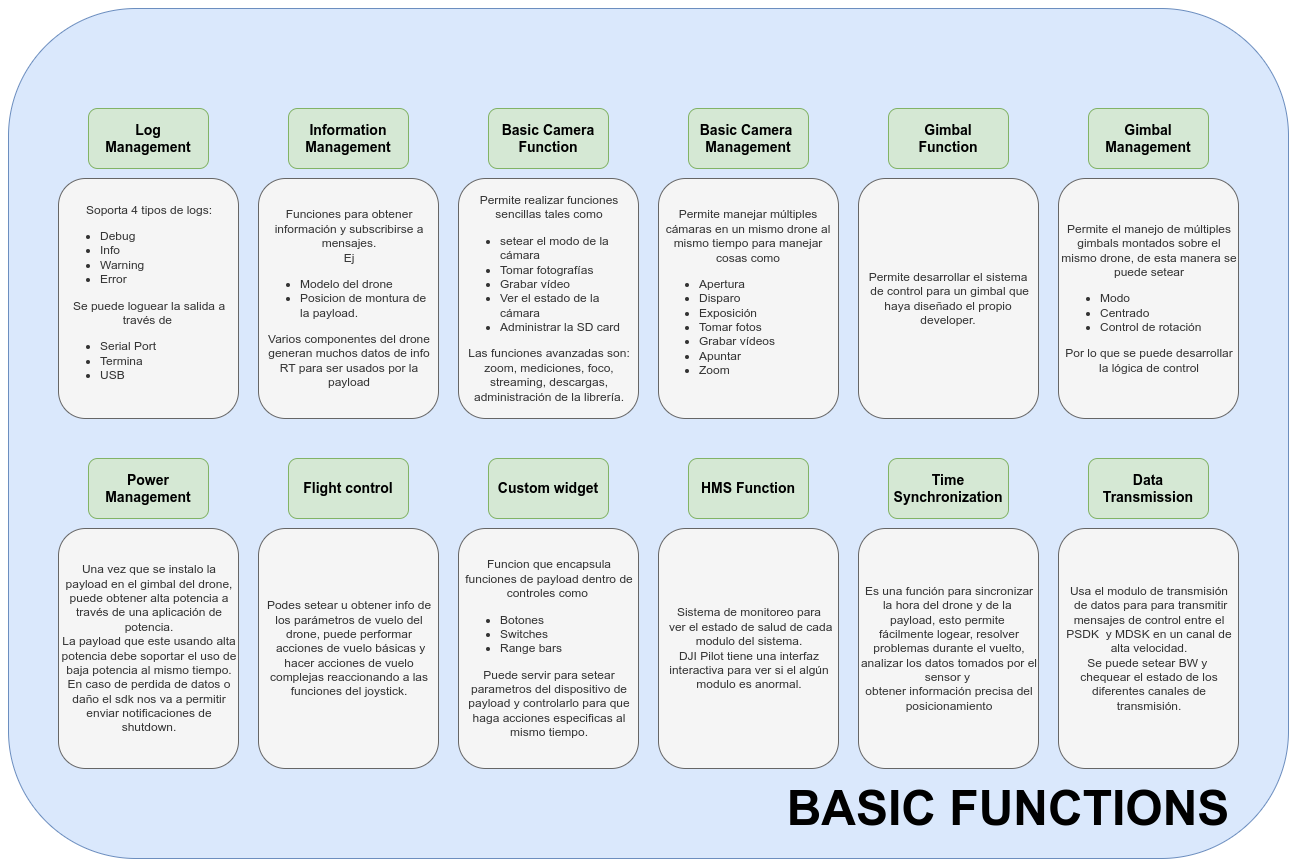
\includegraphics[width=\linewidth]{images/basic_function.png}
    \caption{Fig. 5.1: Basic Function}
  \end{subfigure}
  \begin{subfigure}[b]{0.45\linewidth}
    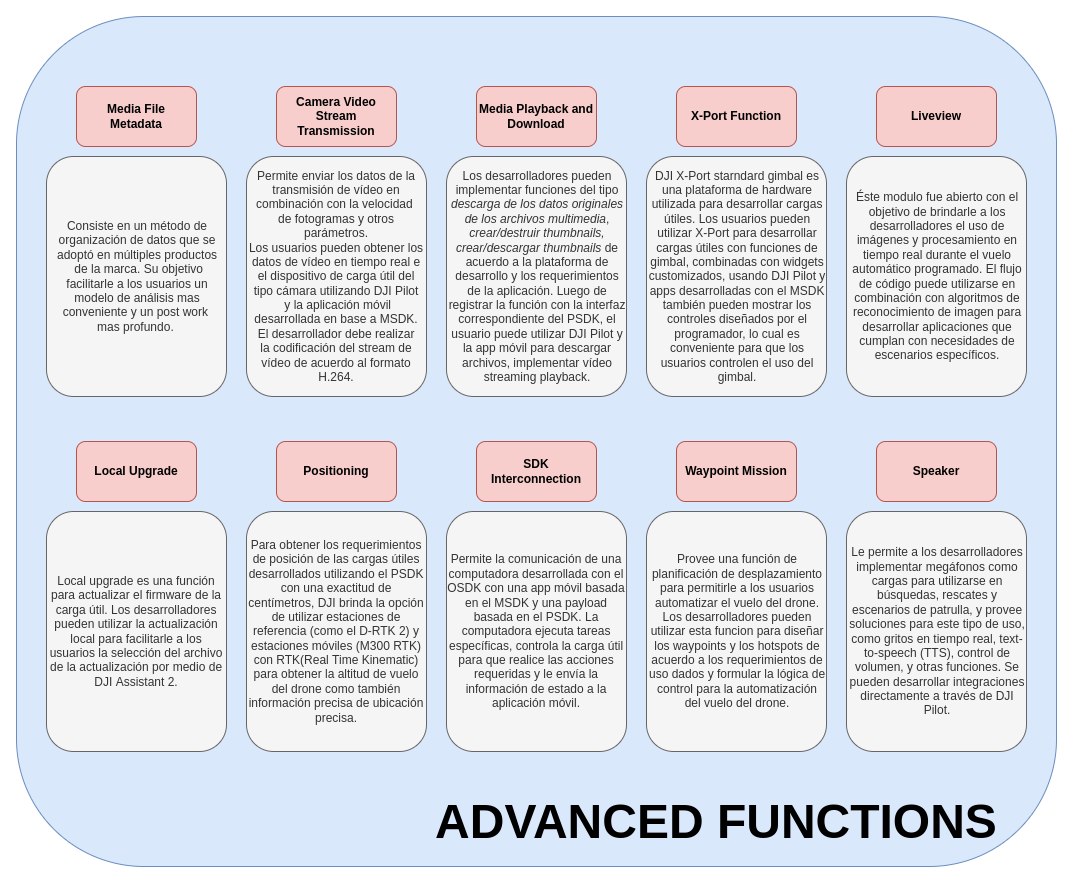
\includegraphics[width=\linewidth]{images/advanced_function.png}
    \caption{Fig. 5.2: Advanced Function}
  \end{subfigure}
\end{figure}

\subsection{PyCom}

\subsection{UART}
\end{document}